\section{Experimental Results}
\label{sec:result}
%%% First Steps and Evaluation (10 points):
%Were the first steps described in the project proposal completed?
%Are there nontrivial preliminary results in terms of system performance or data collection (if data collection is a significant part of the project)?
%Is the interpretation of these results careful and correct?
%Is there an assessment of where the project stands?
%Are next steps clear, including any course corrections based on preliminary results?

We have successfully completed the first steps in the proposal.
We implemented a deep learning neural network using Matlab and then
switched to python because python has a nice deep learning library,
Theano.

Using the python library Theano, we added noise to Logistic Regression
model and Multi-layer Logistic Regression(MLP) model.
As a first step, we have only added noise from binomial and gaussian
distribution. Adding noise of other distributions will be studied later.

In Logistic Regression Model, we added noise to the learning rate.
To be more specific, the weight is updated as

\begin{center}
$W_{new} = W_{old} - learningRateBinomial * \bigtriangledown_{W}$
$W_{new} = W_{old} - learningRateGaussian * \bigtriangledown_{W}$
\end{center}

where $learningRateBinomial$ is a matrix with entries from a binomial
distribution $Bin(1,0.5)$ and $learningRateGaussin$ is a matrix with entries
from a gaussian distribution $\mathcal{N}(0.26,0.13)$.

Our experiments show that adding noise to learning rate can indeed
improve accuracy of the model.

\begin{figure}[t]
\centering
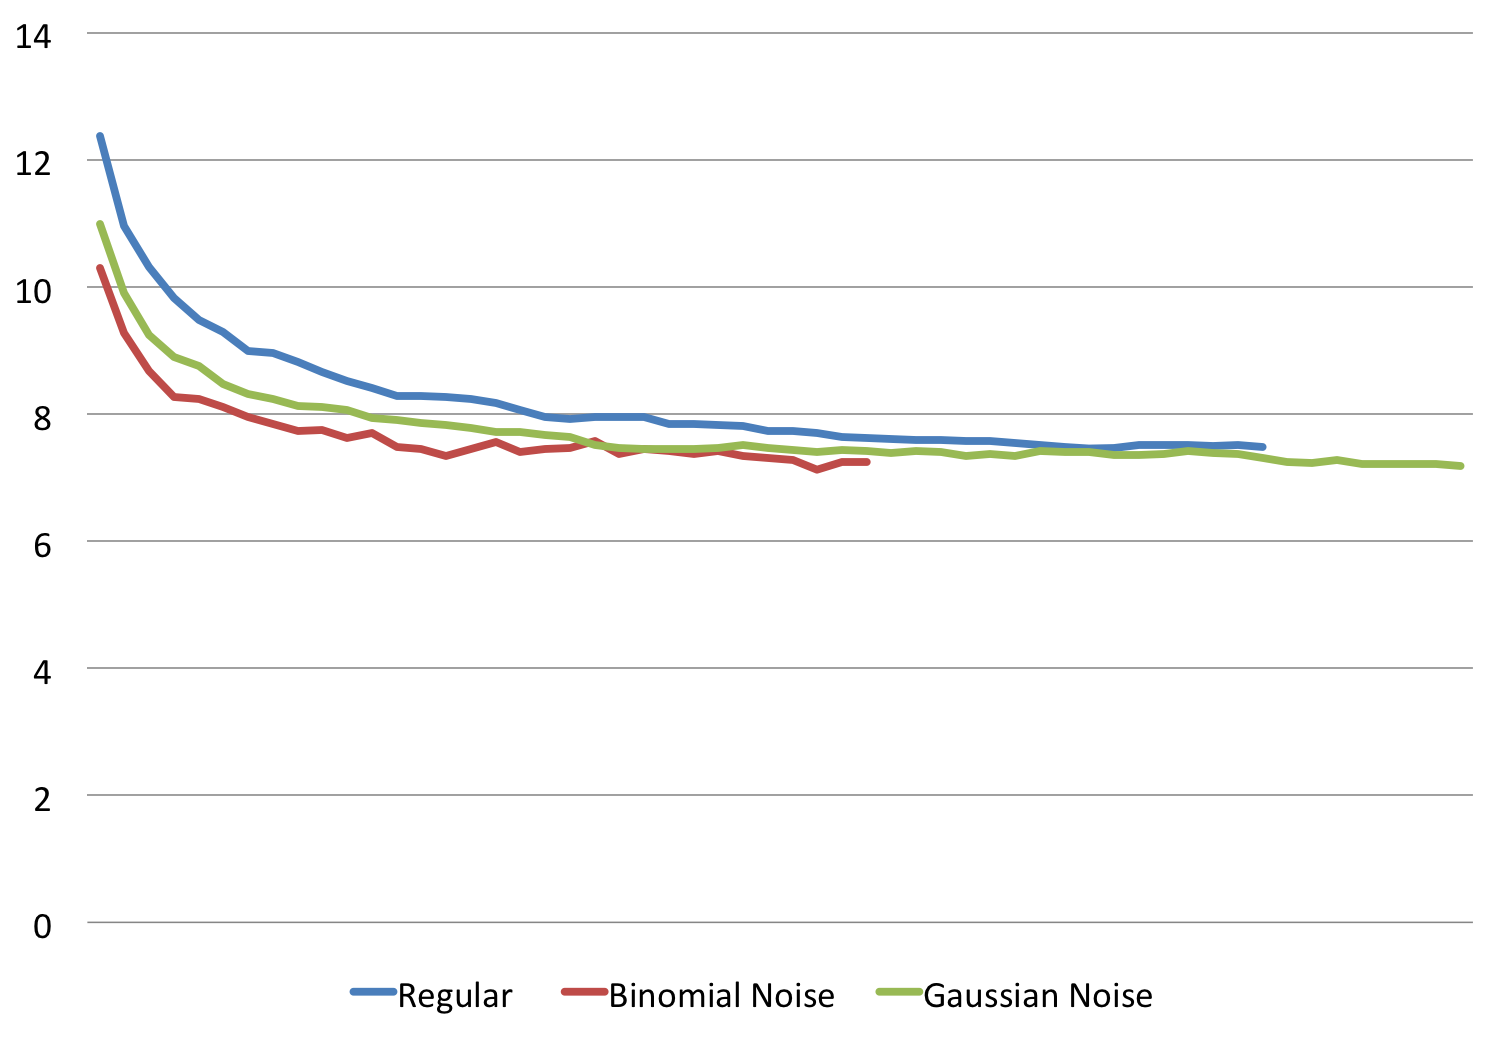
\includegraphics[width=215pt]{figs/logistic_sgd_all.png}
\caption{Logistic Regression with Noise}
\label{fig:logistic-sgd}
\end{figure}

Figure~\ref{fig:logistic-sgd} shows the accuracy of three models.
The blue line shows the test error rate of a regular Logistic Regression Model.
The green line shows the test error rate of a Logistic Regression Model with
gaussian noise added to the learning rate.  The red line shows the test error
rate of a Logistic Regression Model with binomial noise added the learning rate.
The models with noise outperform the regular model through the whole training
process.  We also observe that the red line is less smooth than the green line.
This behavior is expected since if the learning rate is from a binomial
distribution, it is possible that during the gradient descent we will step back
several times.

In general, the model with binomial noise converges faster than the model
with gaussian noise, but eventually they have the same best test error
rate.

